\subsection{Постановка задачи}
1.2. Реализовать метод прогонки в виде программы, задавая в качестве входных данных ненулевые элементы матрицы системы и вектор правых частей. Используя разработанное программное обеспечение, решить СЛАУ с трехдиагональной матрицей. 

{\bfseries Вариант:} 19
\begin{equation}
        \left\{ 
        \begin{array}{ll} 
        10x_1 - x_2 = 16 \\
        -8x_1 + 16x_2 + x_3 = -110\\
        6x_2 - 16x_3 + 6x_4 = 24\\
        -8x_3 + 16x_4 - 5x_5 = -3\\
        5x_4 - 13x_5 = 87\\
        \end{array}\right.
\end{equation}
\pagebreak

\subsection{Результаты работы}

\begin{figure}[h!]
\centering
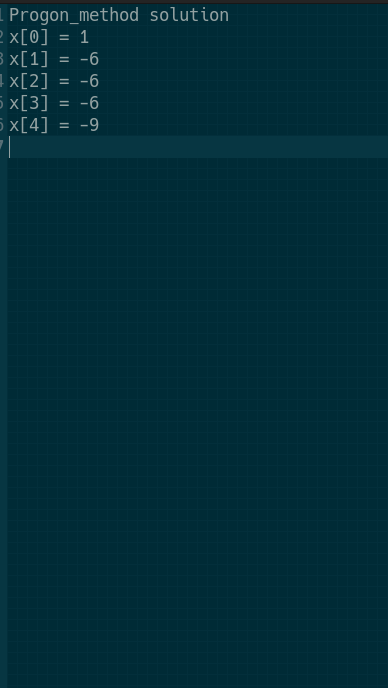
\includegraphics[width=.5\textwidth]{lab1.2}
\caption{Вывод в консоли}
\end{figure}
\pagebreak

\vfill

\subsection{Исходный код}

\lstinputlisting[title=\texttt{Lab1.2.cpp}]{../stud/saifullin/task1.2/Lab1.2.cpp}
\pagebreak
